\documentclass[12pt]{report}
\usepackage{../mystyle}
\begin{document}
\boldmath
\fancyhead[L]{Homework 4.}
\fancyhead[C]{Ordered sets in Data Analysis}
\fancyhead[R]{Ryabykin Aleksey}
\begin{problem}{}
    {\begin{wrapfigure}{r}{0.3\columnwidth} 
        \begin{flushright}
        \begin{tabular}{c|c|c|c|c|}
            & a & b & c & d \\ \hline
          1 &  & $\times$ & $\times$ & $\times$ \\ \hline
          2 & $\times$ & $\times$ & $\times$ &  \\ \hline
          3 &  & $\times$ & $\times$ &  \\ \hline
          4 & $\times$ &  &  & $\times$ \\ \hline
          5 & $\times$ & $\times$ &  & $\times$ \\ \hline
          \end{tabular}
        \end{flushright}
   \end{wrapfigure}
   For the context given by the following table:
   \subsubsection*{CONSTRUCT}
\begin{enumerate*}
    \item All concepts using CbO;
    \item Diagram of the concept lattice;
    \item Generator cover of implications and proper premise base of implications;
    \item Generator basis of association rules with $\conf \geq \dfrac{1}{3}$ and $\supp \geq \dfrac{1}{4}$ (using concept lattice diagram).
\end{enumerate*}}
\end{problem}
\begin{solution}
    \begin{enumerate}
        \item CbO 
    \begin{figure}[H]
        \centering
        \vspace*{-1cm}

        \tikzset{every picture/.style={line width=0.75pt}} %set default line width to 0.75pt        

        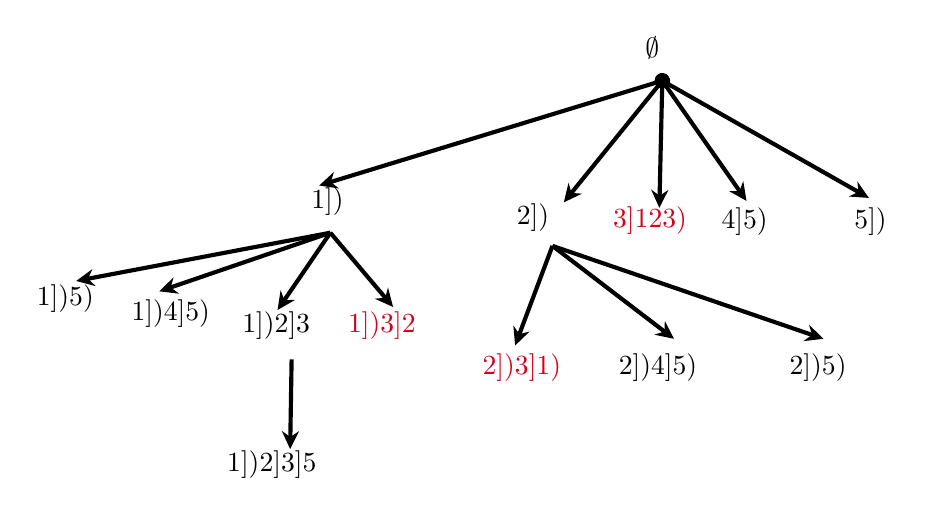
\begin{tikzpicture}[x=0.75pt,y=0.75pt,yscale=-1,xscale=1]
        %uncomment if require: \path (0,300); %set diagram left start at 0, and has height of 300
        
        %Straight Lines [id:da9974037089663628] 
        \draw [line width=1.5]    (300.48,49.9) -- (255.56,105.37) ;
        \draw [shift={(253.05,108.48)}, rotate = 309] [fill={rgb, 255:red, 0; green, 0; blue, 0 }  ][line width=0.08]  [draw opacity=0] (8.75,-4.2) -- (0,0) -- (8.75,4.2) -- (5.81,0) -- cycle    ;
        \draw [shift={(300.48,49.9)}, rotate = 129] [color={rgb, 255:red, 0; green, 0; blue, 0 }  ][fill={rgb, 255:red, 0; green, 0; blue, 0 }  ][line width=1.5]      (0, 0) circle [x radius= 2.61, y radius= 2.61]   ;
        %Straight Lines [id:da017856243455980803] 
        \draw [line width=1.5]    (139,99.21) -- (300.48,49.9) ;
        \draw [shift={(300.48,49.9)}, rotate = 343.02] [color={rgb, 255:red, 0; green, 0; blue, 0 }  ][fill={rgb, 255:red, 0; green, 0; blue, 0 }  ][line width=1.5]      (0, 0) circle [x radius= 2.61, y radius= 2.61]   ;
        \draw [shift={(135.17,100.38)}, rotate = 343.02] [fill={rgb, 255:red, 0; green, 0; blue, 0 }  ][line width=0.08]  [draw opacity=0] (8.75,-4.2) -- (0,0) -- (8.75,4.2) -- (5.81,0) -- cycle    ;
        %Straight Lines [id:da6079745686487605] 
        \draw [line width=1.5]    (300.48,49.9) -- (299.14,107.14) ;
        \draw [shift={(299.05,111.14)}, rotate = 271.34] [fill={rgb, 255:red, 0; green, 0; blue, 0 }  ][line width=0.08]  [draw opacity=0] (8.75,-4.2) -- (0,0) -- (8.75,4.2) -- (5.81,0) -- cycle    ;
        \draw [shift={(300.48,49.9)}, rotate = 91.34] [color={rgb, 255:red, 0; green, 0; blue, 0 }  ][fill={rgb, 255:red, 0; green, 0; blue, 0 }  ][line width=1.5]      (0, 0) circle [x radius= 2.61, y radius= 2.61]   ;
        %Straight Lines [id:da2599088471671398] 
        \draw [line width=1.5]    (300.48,49.9) -- (338.75,104.53) ;
        \draw [shift={(341.05,107.81)}, rotate = 234.98] [fill={rgb, 255:red, 0; green, 0; blue, 0 }  ][line width=0.08]  [draw opacity=0] (8.75,-4.2) -- (0,0) -- (8.75,4.2) -- (5.81,0) -- cycle    ;
        \draw [shift={(300.48,49.9)}, rotate = 54.98] [color={rgb, 255:red, 0; green, 0; blue, 0 }  ][fill={rgb, 255:red, 0; green, 0; blue, 0 }  ][line width=1.5]      (0, 0) circle [x radius= 2.61, y radius= 2.61]   ;
        %Straight Lines [id:da23442481795162684] 
        \draw [line width=1.5]    (396.52,104.38) -- (300.48,49.9) ;
        \draw [shift={(300.48,49.9)}, rotate = 209.56] [color={rgb, 255:red, 0; green, 0; blue, 0 }  ][fill={rgb, 255:red, 0; green, 0; blue, 0 }  ][line width=1.5]      (0, 0) circle [x radius= 2.61, y radius= 2.61]   ;
        \draw [shift={(400,106.36)}, rotate = 209.56] [fill={rgb, 255:red, 0; green, 0; blue, 0 }  ][line width=0.08]  [draw opacity=0] (8.75,-4.2) -- (0,0) -- (8.75,4.2) -- (5.81,0) -- cycle    ;
        %Straight Lines [id:da818600729369954] 
        \draw [line width=1.5]    (230.97,173.72) -- (247.55,129.48) ;
        \draw [shift={(229.57,177.46)}, rotate = 290.54] [fill={rgb, 255:red, 0; green, 0; blue, 0 }  ][line width=0.08]  [draw opacity=0] (8.75,-4.2) -- (0,0) -- (8.75,4.2) -- (5.81,0) -- cycle    ;
        %Straight Lines [id:da7370208794775721] 
        \draw [line width=1.5]    (302.92,171.81) -- (247.55,129.48) ;
        \draw [shift={(306.1,174.24)}, rotate = 217.4] [fill={rgb, 255:red, 0; green, 0; blue, 0 }  ][line width=0.08]  [draw opacity=0] (8.75,-4.2) -- (0,0) -- (8.75,4.2) -- (5.81,0) -- cycle    ;
        %Straight Lines [id:da357630503079156] 
        \draw [line width=1.5]    (374.31,172.94) -- (247.55,129.48) ;
        \draw [shift={(378.1,174.24)}, rotate = 198.93] [fill={rgb, 255:red, 0; green, 0; blue, 0 }  ][line width=0.08]  [draw opacity=0] (8.75,-4.2) -- (0,0) -- (8.75,4.2) -- (5.81,0) -- cycle    ;
        %Straight Lines [id:da28171521233091257] 
        \draw [line width=1.5]    (117.37,157.08) -- (140.55,123.14) ;
        \draw [shift={(115.11,160.38)}, rotate = 304.33] [fill={rgb, 255:red, 0; green, 0; blue, 0 }  ][line width=0.08]  [draw opacity=0] (8.75,-4.2) -- (0,0) -- (8.75,4.2) -- (5.81,0) -- cycle    ;
        %Straight Lines [id:da2968565474164482] 
        \draw [line width=1.5]    (121.24,223.38) -- (121.88,184.14) ;
        \draw [shift={(121.17,227.38)}, rotate = 270.94] [fill={rgb, 255:red, 0; green, 0; blue, 0 }  ][line width=0.08]  [draw opacity=0] (8.75,-4.2) -- (0,0) -- (8.75,4.2) -- (5.81,0) -- cycle    ;
        %Straight Lines [id:da826837142699705] 
        \draw [line width=1.5]    (22.04,145.63) -- (140.55,123.14) ;
        \draw [shift={(18.11,146.38)}, rotate = 349.25] [fill={rgb, 255:red, 0; green, 0; blue, 0 }  ][line width=0.08]  [draw opacity=0] (8.75,-4.2) -- (0,0) -- (8.75,4.2) -- (5.81,0) -- cycle    ;
        %Straight Lines [id:da1623703084250543] 
        \draw [line width=1.5]    (168.18,155.85) -- (140.55,123.14) ;
        \draw [shift={(170.76,158.9)}, rotate = 229.81] [fill={rgb, 255:red, 0; green, 0; blue, 0 }  ][line width=0.08]  [draw opacity=0] (8.75,-4.2) -- (0,0) -- (8.75,4.2) -- (5.81,0) -- cycle    ;
        %Straight Lines [id:da053037753382565445] 
        \draw [line width=1.5]    (61.9,150.08) -- (140.55,123.14) ;
        \draw [shift={(58.11,151.38)}, rotate = 341.09] [fill={rgb, 255:red, 0; green, 0; blue, 0 }  ][line width=0.08]  [draw opacity=0] (8.75,-4.2) -- (0,0) -- (8.75,4.2) -- (5.81,0) -- cycle    ;
        
        % Text Node
        \draw (143.39,107.96) node   [align=left] {\begin{minipage}[lt]{18.02pt}\setlength\topsep{0pt}
        1])
        \end{minipage}};
        % Text Node
        \draw (242.39,115.96) node   [align=left] {\begin{minipage}[lt]{18.02pt}\setlength\topsep{0pt}
        2])
        \end{minipage}};
        % Text Node
        \draw (299.05,117.14) node  [color={rgb, 255:red, 208; green, 2; blue, 27 }  ,opacity=1 ] [align=left] {\begin{minipage}[lt]{33.37pt}\setlength\topsep{0pt}
        3]123)
        \end{minipage}};
        % Text Node
        \draw (341.05,117.81) node   [align=left] {\begin{minipage}[lt]{18.02pt}\setlength\topsep{0pt}
        4]5)
        \end{minipage}};
        % Text Node
        \draw (405.07,117.96) node   [align=left] {\begin{minipage}[lt]{18.02pt}\setlength\topsep{0pt}
        5])
        \end{minipage}};
        % Text Node
        \draw (120.16,168) node   [align=left] {\begin{minipage}[lt]{33pt}\setlength\topsep{0pt}
        1])2]3
        \end{minipage}};
        % Text Node
        \draw (240.16,188) node  [color={rgb, 255:red, 208; green, 2; blue, 27 }  ,opacity=1 ] [align=left] {\begin{minipage}[lt]{39.35pt}\setlength\topsep{0pt}
        2])3]1)
        \end{minipage}};
        % Text Node
        \draw (304.83,188) node   [align=left] {\begin{minipage}[lt]{37.99pt}\setlength\topsep{0pt}
        2])4]5)
        \end{minipage}};
        % Text Node
        \draw (383.83,188) node   [align=left] {\begin{minipage}[lt]{33pt}\setlength\topsep{0pt}
        2])5)
        \end{minipage}};
        % Text Node
        \draw (119.82,235) node   [align=left] {\begin{minipage}[lt]{43.44pt}\setlength\topsep{0pt}
        1])2]3]5
        \end{minipage}};
        % Text Node
        \draw (171.1,168) node  [color={rgb, 255:red, 208; green, 2; blue, 27 }  ,opacity=1 ] [align=left] {\begin{minipage}[lt]{33pt}\setlength\topsep{0pt}
        1])3]2
        \end{minipage}};
        % Text Node
        \draw (66.76,162) node   [align=left] {\begin{minipage}[lt]{33pt}\setlength\topsep{0pt}
        1])4]5)
        \end{minipage}};
        % Text Node
        \draw (21.16,155) node   [align=left] {\begin{minipage}[lt]{33pt}\setlength\topsep{0pt}
        1])5)
        \end{minipage}};
        % Text Node
        \draw (301.12,34.16) node   [align=left] {\begin{minipage}[lt]{13.24pt}\setlength\topsep{0pt}
        $\displaystyle \emptyset $
        \end{minipage}};        
        \end{tikzpicture}        
    \end{figure}
    All concepts 
    \begin{multicols}{3}
        \begin{itemize}
            \item $(\emptyset, \{a,b,c,d\})$;
            \item $(1, \{b,c,d\})$;
            \item $(2, \{a,b,c\})$;
            \item $(5, \{a,b,d\})$;
            \item $(\left\{1,5\right\}, \{b,d\})$;
            \item $(\left\{2,5\right\}, \{a,b\})$;
            \item $(\left\{4,5\right\}, \{a,d\})$;
            \item $(\left\{1,2,3\right\}, \{b,c\})$;
            \item $(\left\{1,4, 5\right\}, \{d\})$;
            \item $(\left\{2,4,5\right\}, \{a\})$;
            \item $(\left\{1,2,3,5\right\}, \{b\})$;
            \item $(\left\{1,2,3,4,5\right\}, \{\emptyset\})$;
        \end{itemize}
    \end{multicols}
    \item Concept lattice:
    \begin{figure}[H]
        \centering
        

\tikzset{every picture/.style={line width=0.75pt}} %set default line width to 0.75pt        

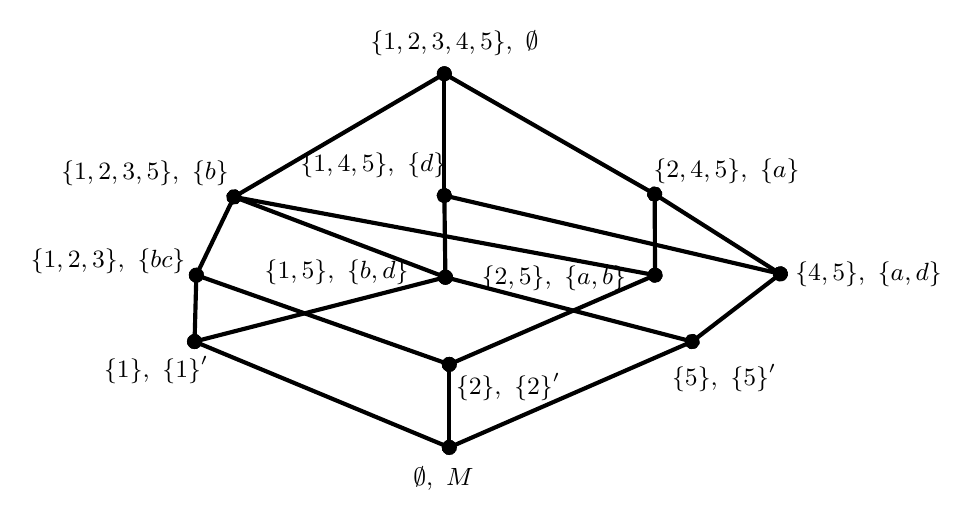
\begin{tikzpicture}[x=0.75pt,y=0.75pt,yscale=-1,xscale=1]
%uncomment if require: \path (0,244); %set diagram left start at 0, and has height of 244

%Straight Lines [id:da7860117304011858] 
\draw [line width=1.5]    (219.48,30.9) -- (320.81,88.9) ;
\draw [shift={(320.81,88.9)}, rotate = 29.79] [color={rgb, 255:red, 0; green, 0; blue, 0 }  ][fill={rgb, 255:red, 0; green, 0; blue, 0 }  ][line width=1.5]      (0, 0) circle [x radius= 2.61, y radius= 2.61]   ;
\draw [shift={(219.48,30.9)}, rotate = 29.79] [color={rgb, 255:red, 0; green, 0; blue, 0 }  ][fill={rgb, 255:red, 0; green, 0; blue, 0 }  ][line width=1.5]      (0, 0) circle [x radius= 2.61, y radius= 2.61]   ;
%Straight Lines [id:da8370249623404562] 
\draw [line width=1.5]    (118.14,90.24) -- (219.48,30.9) ;
\draw [shift={(219.48,30.9)}, rotate = 329.65] [color={rgb, 255:red, 0; green, 0; blue, 0 }  ][fill={rgb, 255:red, 0; green, 0; blue, 0 }  ][line width=1.5]      (0, 0) circle [x radius= 2.61, y radius= 2.61]   ;
\draw [shift={(118.14,90.24)}, rotate = 329.65] [color={rgb, 255:red, 0; green, 0; blue, 0 }  ][fill={rgb, 255:red, 0; green, 0; blue, 0 }  ][line width=1.5]      (0, 0) circle [x radius= 2.61, y radius= 2.61]   ;
%Straight Lines [id:da9193891755773385] 
\draw [line width=1.5]    (219.48,30.9) -- (219.48,89.57) ;
\draw [shift={(219.48,89.57)}, rotate = 90] [color={rgb, 255:red, 0; green, 0; blue, 0 }  ][fill={rgb, 255:red, 0; green, 0; blue, 0 }  ][line width=1.5]      (0, 0) circle [x radius= 2.61, y radius= 2.61]   ;
\draw [shift={(219.48,30.9)}, rotate = 90] [color={rgb, 255:red, 0; green, 0; blue, 0 }  ][fill={rgb, 255:red, 0; green, 0; blue, 0 }  ][line width=1.5]      (0, 0) circle [x radius= 2.61, y radius= 2.61]   ;
%Straight Lines [id:da05172661742722928] 
\draw [line width=1.5]    (381.38,127.31) -- (320.81,88.9) ;
\draw [shift={(320.81,88.9)}, rotate = 212.38] [color={rgb, 255:red, 0; green, 0; blue, 0 }  ][fill={rgb, 255:red, 0; green, 0; blue, 0 }  ][line width=1.5]      (0, 0) circle [x radius= 2.61, y radius= 2.61]   ;
\draw [shift={(381.38,127.31)}, rotate = 212.38] [color={rgb, 255:red, 0; green, 0; blue, 0 }  ][fill={rgb, 255:red, 0; green, 0; blue, 0 }  ][line width=1.5]      (0, 0) circle [x radius= 2.61, y radius= 2.61]   ;
%Straight Lines [id:da7783392092706243] 
\draw [line width=1.5]    (321,127.93) -- (320.81,88.9) ;
\draw [shift={(320.81,88.9)}, rotate = 269.72] [color={rgb, 255:red, 0; green, 0; blue, 0 }  ][fill={rgb, 255:red, 0; green, 0; blue, 0 }  ][line width=1.5]      (0, 0) circle [x radius= 2.61, y radius= 2.61]   ;
\draw [shift={(321,127.93)}, rotate = 269.72] [color={rgb, 255:red, 0; green, 0; blue, 0 }  ][fill={rgb, 255:red, 0; green, 0; blue, 0 }  ][line width=1.5]      (0, 0) circle [x radius= 2.61, y radius= 2.61]   ;
%Straight Lines [id:da4978706843782126] 
\draw [line width=1.5]    (381.38,127.31) -- (219.48,89.57) ;
\draw [shift={(219.48,89.57)}, rotate = 193.12] [color={rgb, 255:red, 0; green, 0; blue, 0 }  ][fill={rgb, 255:red, 0; green, 0; blue, 0 }  ][line width=1.5]      (0, 0) circle [x radius= 2.61, y radius= 2.61]   ;
\draw [shift={(381.38,127.31)}, rotate = 193.12] [color={rgb, 255:red, 0; green, 0; blue, 0 }  ][fill={rgb, 255:red, 0; green, 0; blue, 0 }  ][line width=1.5]      (0, 0) circle [x radius= 2.61, y radius= 2.61]   ;
%Straight Lines [id:da17523783533616832] 
\draw [line width=1.5]    (321,127.93) -- (118.14,90.24) ;
\draw [shift={(118.14,90.24)}, rotate = 190.53] [color={rgb, 255:red, 0; green, 0; blue, 0 }  ][fill={rgb, 255:red, 0; green, 0; blue, 0 }  ][line width=1.5]      (0, 0) circle [x radius= 2.61, y radius= 2.61]   ;
\draw [shift={(321,127.93)}, rotate = 190.53] [color={rgb, 255:red, 0; green, 0; blue, 0 }  ][fill={rgb, 255:red, 0; green, 0; blue, 0 }  ][line width=1.5]      (0, 0) circle [x radius= 2.61, y radius= 2.61]   ;
%Straight Lines [id:da017002821841653137] 
\draw [line width=1.5]    (220,128.93) -- (219.48,89.57) ;
\draw [shift={(219.48,89.57)}, rotate = 269.24] [color={rgb, 255:red, 0; green, 0; blue, 0 }  ][fill={rgb, 255:red, 0; green, 0; blue, 0 }  ][line width=1.5]      (0, 0) circle [x radius= 2.61, y radius= 2.61]   ;
\draw [shift={(220,128.93)}, rotate = 269.24] [color={rgb, 255:red, 0; green, 0; blue, 0 }  ][fill={rgb, 255:red, 0; green, 0; blue, 0 }  ][line width=1.5]      (0, 0) circle [x radius= 2.61, y radius= 2.61]   ;
%Straight Lines [id:da2144479444113474] 
\draw [line width=1.5]    (220,128.93) -- (118.14,90.24) ;
\draw [shift={(118.14,90.24)}, rotate = 200.8] [color={rgb, 255:red, 0; green, 0; blue, 0 }  ][fill={rgb, 255:red, 0; green, 0; blue, 0 }  ][line width=1.5]      (0, 0) circle [x radius= 2.61, y radius= 2.61]   ;
\draw [shift={(220,128.93)}, rotate = 200.8] [color={rgb, 255:red, 0; green, 0; blue, 0 }  ][fill={rgb, 255:red, 0; green, 0; blue, 0 }  ][line width=1.5]      (0, 0) circle [x radius= 2.61, y radius= 2.61]   ;
%Straight Lines [id:da5251675369412507] 
\draw [line width=1.5]    (100,127.93) -- (118.14,90.24) ;
\draw [shift={(118.14,90.24)}, rotate = 295.7] [color={rgb, 255:red, 0; green, 0; blue, 0 }  ][fill={rgb, 255:red, 0; green, 0; blue, 0 }  ][line width=1.5]      (0, 0) circle [x radius= 2.61, y radius= 2.61]   ;
\draw [shift={(100,127.93)}, rotate = 295.7] [color={rgb, 255:red, 0; green, 0; blue, 0 }  ][fill={rgb, 255:red, 0; green, 0; blue, 0 }  ][line width=1.5]      (0, 0) circle [x radius= 2.61, y radius= 2.61]   ;
%Straight Lines [id:da07510840772576688] 
\draw [line width=1.5]    (100,127.93) -- (99.14,159.93) ;
\draw [shift={(99.14,159.93)}, rotate = 91.53] [color={rgb, 255:red, 0; green, 0; blue, 0 }  ][fill={rgb, 255:red, 0; green, 0; blue, 0 }  ][line width=1.5]      (0, 0) circle [x radius= 2.61, y radius= 2.61]   ;
\draw [shift={(100,127.93)}, rotate = 91.53] [color={rgb, 255:red, 0; green, 0; blue, 0 }  ][fill={rgb, 255:red, 0; green, 0; blue, 0 }  ][line width=1.5]      (0, 0) circle [x radius= 2.61, y radius= 2.61]   ;
%Straight Lines [id:da7583268397655496] 
\draw [line width=1.5]    (99.14,159.93) -- (221.86,210.93) ;
\draw [shift={(221.86,210.93)}, rotate = 22.57] [color={rgb, 255:red, 0; green, 0; blue, 0 }  ][fill={rgb, 255:red, 0; green, 0; blue, 0 }  ][line width=1.5]      (0, 0) circle [x radius= 2.61, y radius= 2.61]   ;
\draw [shift={(99.14,159.93)}, rotate = 22.57] [color={rgb, 255:red, 0; green, 0; blue, 0 }  ][fill={rgb, 255:red, 0; green, 0; blue, 0 }  ][line width=1.5]      (0, 0) circle [x radius= 2.61, y radius= 2.61]   ;
%Straight Lines [id:da16942430715237422] 
\draw [line width=1.5]    (220,128.93) -- (99.14,159.93) ;
\draw [shift={(99.14,159.93)}, rotate = 165.61] [color={rgb, 255:red, 0; green, 0; blue, 0 }  ][fill={rgb, 255:red, 0; green, 0; blue, 0 }  ][line width=1.5]      (0, 0) circle [x radius= 2.61, y radius= 2.61]   ;
\draw [shift={(220,128.93)}, rotate = 165.61] [color={rgb, 255:red, 0; green, 0; blue, 0 }  ][fill={rgb, 255:red, 0; green, 0; blue, 0 }  ][line width=1.5]      (0, 0) circle [x radius= 2.61, y radius= 2.61]   ;
%Straight Lines [id:da4531823280908993] 
\draw [line width=1.5]    (100,127.93) -- (221.86,170.93) ;
\draw [shift={(221.86,170.93)}, rotate = 19.44] [color={rgb, 255:red, 0; green, 0; blue, 0 }  ][fill={rgb, 255:red, 0; green, 0; blue, 0 }  ][line width=1.5]      (0, 0) circle [x radius= 2.61, y radius= 2.61]   ;
\draw [shift={(100,127.93)}, rotate = 19.44] [color={rgb, 255:red, 0; green, 0; blue, 0 }  ][fill={rgb, 255:red, 0; green, 0; blue, 0 }  ][line width=1.5]      (0, 0) circle [x radius= 2.61, y radius= 2.61]   ;
%Straight Lines [id:da9126977761562813] 
\draw [line width=1.5]    (321,127.93) -- (221.86,170.93) ;
\draw [shift={(221.86,170.93)}, rotate = 156.55] [color={rgb, 255:red, 0; green, 0; blue, 0 }  ][fill={rgb, 255:red, 0; green, 0; blue, 0 }  ][line width=1.5]      (0, 0) circle [x radius= 2.61, y radius= 2.61]   ;
\draw [shift={(321,127.93)}, rotate = 156.55] [color={rgb, 255:red, 0; green, 0; blue, 0 }  ][fill={rgb, 255:red, 0; green, 0; blue, 0 }  ][line width=1.5]      (0, 0) circle [x radius= 2.61, y radius= 2.61]   ;
%Straight Lines [id:da7031077454428647] 
\draw [line width=1.5]    (220,128.93) -- (338.86,159.93) ;
\draw [shift={(338.86,159.93)}, rotate = 14.62] [color={rgb, 255:red, 0; green, 0; blue, 0 }  ][fill={rgb, 255:red, 0; green, 0; blue, 0 }  ][line width=1.5]      (0, 0) circle [x radius= 2.61, y radius= 2.61]   ;
\draw [shift={(220,128.93)}, rotate = 14.62] [color={rgb, 255:red, 0; green, 0; blue, 0 }  ][fill={rgb, 255:red, 0; green, 0; blue, 0 }  ][line width=1.5]      (0, 0) circle [x radius= 2.61, y radius= 2.61]   ;
%Straight Lines [id:da5796281071141236] 
\draw [line width=1.5]    (381.38,127.31) -- (338.86,159.93) ;
\draw [shift={(338.86,159.93)}, rotate = 142.51] [color={rgb, 255:red, 0; green, 0; blue, 0 }  ][fill={rgb, 255:red, 0; green, 0; blue, 0 }  ][line width=1.5]      (0, 0) circle [x radius= 2.61, y radius= 2.61]   ;
\draw [shift={(381.38,127.31)}, rotate = 142.51] [color={rgb, 255:red, 0; green, 0; blue, 0 }  ][fill={rgb, 255:red, 0; green, 0; blue, 0 }  ][line width=1.5]      (0, 0) circle [x radius= 2.61, y radius= 2.61]   ;
%Straight Lines [id:da8855504557668914] 
\draw [line width=1.5]    (221.86,170.93) -- (221.86,210.93) ;
\draw [shift={(221.86,210.93)}, rotate = 90] [color={rgb, 255:red, 0; green, 0; blue, 0 }  ][fill={rgb, 255:red, 0; green, 0; blue, 0 }  ][line width=1.5]      (0, 0) circle [x radius= 2.61, y radius= 2.61]   ;
\draw [shift={(221.86,170.93)}, rotate = 90] [color={rgb, 255:red, 0; green, 0; blue, 0 }  ][fill={rgb, 255:red, 0; green, 0; blue, 0 }  ][line width=1.5]      (0, 0) circle [x radius= 2.61, y radius= 2.61]   ;
%Straight Lines [id:da6357079262022591] 
\draw [line width=1.5]    (338.86,159.93) -- (221.86,210.93) ;
\draw [shift={(221.86,210.93)}, rotate = 156.45] [color={rgb, 255:red, 0; green, 0; blue, 0 }  ][fill={rgb, 255:red, 0; green, 0; blue, 0 }  ][line width=1.5]      (0, 0) circle [x radius= 2.61, y radius= 2.61]   ;
\draw [shift={(338.86,159.93)}, rotate = 156.45] [color={rgb, 255:red, 0; green, 0; blue, 0 }  ][fill={rgb, 255:red, 0; green, 0; blue, 0 }  ][line width=1.5]      (0, 0) circle [x radius= 2.61, y radius= 2.61]   ;

% Text Node
\draw (182.67,8.97) node [anchor=north west][inner sep=0.75pt]  [font=\small] [align=left] {$\displaystyle \{1,2,3,4,5\} ,\ \emptyset $};
% Text Node
\draw (149,67.8) node [anchor=north west][inner sep=0.75pt]  [font=\small] [align=left] {$\displaystyle \{1,4,5\} ,\ \{d\}$};
% Text Node
\draw (319,70.8) node [anchor=north west][inner sep=0.75pt]  [font=\small] [align=left] {$\displaystyle \{2,4,5\} ,\ \{a\}$};
% Text Node
\draw (54.33,165.8) node [anchor=north west][inner sep=0.75pt]  [font=\small] [align=left] {$\displaystyle \{1\} ,\ \{1\} '$};
% Text Node
\draw (131.67,119.47) node [anchor=north west][inner sep=0.75pt]  [font=\small] [align=left] {$\displaystyle \{1,5\} ,\ \{b,d\}$};
% Text Node
\draw (203.33,219.13) node [anchor=north west][inner sep=0.75pt]  [font=\small] [align=left] {$\displaystyle \emptyset ,\ M$};
% Text Node
\draw (33.67,71.8) node [anchor=north west][inner sep=0.75pt]  [font=\small] [align=left] {$\displaystyle \{1,2,3,5\} ,\ \{b\}$};
% Text Node
\draw (387.38,120.11) node [anchor=north west][inner sep=0.75pt]  [font=\small] [align=left] {$\displaystyle \{4,5\} ,\ \{a,d\}$};
% Text Node
\draw (236.33,122.13) node [anchor=north west][inner sep=0.75pt]  [font=\small] [align=left] {$\displaystyle \{2,5\} ,\ \{a,b\}$};
% Text Node
\draw (19,113.8) node [anchor=north west][inner sep=0.75pt]  [font=\small] [align=left] {$\displaystyle \{1,2,3\} ,\ \{bc\}$};
% Text Node
\draw (328,169.8) node [anchor=north west][inner sep=0.75pt]  [font=\small] [align=left] {$\displaystyle \{5\} ,\ \{5\} '$};
% Text Node
\draw (223.86,173.73) node [anchor=north west][inner sep=0.75pt]  [font=\small] [align=left] {$\displaystyle \{2\} ,\ \{2\} '$};


\end{tikzpicture}

    \end{figure}
    \item Generation cover of implications ($\text{MinGen} \to \text{MinGen}''$):
    \begin{itemize}
        \item $acd \to abcd$;
        \item $cd \to bcd$;
        \item $ac \to abc$;
        \item $c \to bc$.
    \end{itemize}
    And after simplifications:
    \begin{itemize}
        \item $acd \to b$
        \item $cd \to b$
        \item $ac \to b$
        \item $c \to b$
    \end{itemize}
    After removing duplicates:
    $c \to b$.
    \item Computed conf and supp:
    \begin{figure}[H]
        \centering
        

\tikzset{every picture/.style={line width=0.75pt}} %set default line width to 0.75pt        

\begin{tikzpicture}[x=0.75pt,y=0.75pt,yscale=-1,xscale=1]
%uncomment if require: \path (0,244); %set diagram left start at 0, and has height of 244

%Straight Lines [id:da7860117304011858] 
\draw [line width=1.5]    (219.48,30.9) -- (320.81,88.9) ;
\draw [shift={(320.81,88.9)}, rotate = 29.79] [color={rgb, 255:red, 0; green, 0; blue, 0 }  ][fill={rgb, 255:red, 0; green, 0; blue, 0 }  ][line width=1.5]      (0, 0) circle [x radius= 2.61, y radius= 2.61]   ;
\draw [shift={(219.48,30.9)}, rotate = 29.79] [color={rgb, 255:red, 0; green, 0; blue, 0 }  ][fill={rgb, 255:red, 0; green, 0; blue, 0 }  ][line width=1.5]      (0, 0) circle [x radius= 2.61, y radius= 2.61]   ;
%Straight Lines [id:da8370249623404562] 
\draw [line width=1.5]    (118.14,90.24) -- (219.48,30.9) ;
\draw [shift={(219.48,30.9)}, rotate = 329.65] [color={rgb, 255:red, 0; green, 0; blue, 0 }  ][fill={rgb, 255:red, 0; green, 0; blue, 0 }  ][line width=1.5]      (0, 0) circle [x radius= 2.61, y radius= 2.61]   ;
\draw [shift={(118.14,90.24)}, rotate = 329.65] [color={rgb, 255:red, 0; green, 0; blue, 0 }  ][fill={rgb, 255:red, 0; green, 0; blue, 0 }  ][line width=1.5]      (0, 0) circle [x radius= 2.61, y radius= 2.61]   ;
%Straight Lines [id:da9193891755773385] 
\draw [line width=1.5]    (219.48,30.9) -- (219.48,89.57) ;
\draw [shift={(219.48,89.57)}, rotate = 90] [color={rgb, 255:red, 0; green, 0; blue, 0 }  ][fill={rgb, 255:red, 0; green, 0; blue, 0 }  ][line width=1.5]      (0, 0) circle [x radius= 2.61, y radius= 2.61]   ;
\draw [shift={(219.48,30.9)}, rotate = 90] [color={rgb, 255:red, 0; green, 0; blue, 0 }  ][fill={rgb, 255:red, 0; green, 0; blue, 0 }  ][line width=1.5]      (0, 0) circle [x radius= 2.61, y radius= 2.61]   ;
%Straight Lines [id:da05172661742722928] 
\draw [line width=1.5]    (381.38,127.31) -- (320.81,88.9) ;
\draw [shift={(320.81,88.9)}, rotate = 212.38] [color={rgb, 255:red, 0; green, 0; blue, 0 }  ][fill={rgb, 255:red, 0; green, 0; blue, 0 }  ][line width=1.5]      (0, 0) circle [x radius= 2.61, y radius= 2.61]   ;
\draw [shift={(381.38,127.31)}, rotate = 212.38] [color={rgb, 255:red, 0; green, 0; blue, 0 }  ][fill={rgb, 255:red, 0; green, 0; blue, 0 }  ][line width=1.5]      (0, 0) circle [x radius= 2.61, y radius= 2.61]   ;
%Straight Lines [id:da7783392092706243] 
\draw [line width=1.5]    (321,127.93) -- (320.81,88.9) ;
\draw [shift={(320.81,88.9)}, rotate = 269.72] [color={rgb, 255:red, 0; green, 0; blue, 0 }  ][fill={rgb, 255:red, 0; green, 0; blue, 0 }  ][line width=1.5]      (0, 0) circle [x radius= 2.61, y radius= 2.61]   ;
\draw [shift={(321,127.93)}, rotate = 269.72] [color={rgb, 255:red, 0; green, 0; blue, 0 }  ][fill={rgb, 255:red, 0; green, 0; blue, 0 }  ][line width=1.5]      (0, 0) circle [x radius= 2.61, y radius= 2.61]   ;
%Straight Lines [id:da4978706843782126] 
\draw [line width=1.5]    (381.38,127.31) -- (219.48,89.57) ;
\draw [shift={(219.48,89.57)}, rotate = 193.12] [color={rgb, 255:red, 0; green, 0; blue, 0 }  ][fill={rgb, 255:red, 0; green, 0; blue, 0 }  ][line width=1.5]      (0, 0) circle [x radius= 2.61, y radius= 2.61]   ;
\draw [shift={(381.38,127.31)}, rotate = 193.12] [color={rgb, 255:red, 0; green, 0; blue, 0 }  ][fill={rgb, 255:red, 0; green, 0; blue, 0 }  ][line width=1.5]      (0, 0) circle [x radius= 2.61, y radius= 2.61]   ;
%Straight Lines [id:da17523783533616832] 
\draw [line width=1.5]    (321,127.93) -- (118.14,90.24) ;
\draw [shift={(118.14,90.24)}, rotate = 190.53] [color={rgb, 255:red, 0; green, 0; blue, 0 }  ][fill={rgb, 255:red, 0; green, 0; blue, 0 }  ][line width=1.5]      (0, 0) circle [x radius= 2.61, y radius= 2.61]   ;
\draw [shift={(321,127.93)}, rotate = 190.53] [color={rgb, 255:red, 0; green, 0; blue, 0 }  ][fill={rgb, 255:red, 0; green, 0; blue, 0 }  ][line width=1.5]      (0, 0) circle [x radius= 2.61, y radius= 2.61]   ;
%Straight Lines [id:da017002821841653137] 
\draw [line width=1.5]    (220,128.93) -- (219.48,89.57) ;
\draw [shift={(219.48,89.57)}, rotate = 269.24] [color={rgb, 255:red, 0; green, 0; blue, 0 }  ][fill={rgb, 255:red, 0; green, 0; blue, 0 }  ][line width=1.5]      (0, 0) circle [x radius= 2.61, y radius= 2.61]   ;
\draw [shift={(220,128.93)}, rotate = 269.24] [color={rgb, 255:red, 0; green, 0; blue, 0 }  ][fill={rgb, 255:red, 0; green, 0; blue, 0 }  ][line width=1.5]      (0, 0) circle [x radius= 2.61, y radius= 2.61]   ;
%Straight Lines [id:da2144479444113474] 
\draw [line width=1.5]    (220,128.93) -- (118.14,90.24) ;
\draw [shift={(118.14,90.24)}, rotate = 200.8] [color={rgb, 255:red, 0; green, 0; blue, 0 }  ][fill={rgb, 255:red, 0; green, 0; blue, 0 }  ][line width=1.5]      (0, 0) circle [x radius= 2.61, y radius= 2.61]   ;
\draw [shift={(220,128.93)}, rotate = 200.8] [color={rgb, 255:red, 0; green, 0; blue, 0 }  ][fill={rgb, 255:red, 0; green, 0; blue, 0 }  ][line width=1.5]      (0, 0) circle [x radius= 2.61, y radius= 2.61]   ;
%Straight Lines [id:da5251675369412507] 
\draw [line width=1.5]    (100,127.93) -- (118.14,90.24) ;
\draw [shift={(118.14,90.24)}, rotate = 295.7] [color={rgb, 255:red, 0; green, 0; blue, 0 }  ][fill={rgb, 255:red, 0; green, 0; blue, 0 }  ][line width=1.5]      (0, 0) circle [x radius= 2.61, y radius= 2.61]   ;
\draw [shift={(100,127.93)}, rotate = 295.7] [color={rgb, 255:red, 0; green, 0; blue, 0 }  ][fill={rgb, 255:red, 0; green, 0; blue, 0 }  ][line width=1.5]      (0, 0) circle [x radius= 2.61, y radius= 2.61]   ;

% Text Node
\draw (182.67,8.97) node [anchor=north west][inner sep=0.75pt]  [font=\small] [align=left] {$\displaystyle \{1,2,3,4,5\} ,\ \emptyset $};
% Text Node
\draw (149,67.8) node [anchor=north west][inner sep=0.75pt]  [font=\small] [align=left] {$\displaystyle \{1,4,5\} ,\ \{d\}$};
% Text Node
\draw (319,70.8) node [anchor=north west][inner sep=0.75pt]  [font=\small] [align=left] {$\displaystyle \{2,4,5\} ,\ \{a\}$};
% Text Node
\draw (131.67,119.47) node [anchor=north west][inner sep=0.75pt]  [font=\small] [align=left] {$\displaystyle \{1,5\} ,\ \{b,d\}$};
% Text Node
\draw (33.67,71.8) node [anchor=north west][inner sep=0.75pt]  [font=\small] [align=left] {$\displaystyle \{1,2,3,5\} ,\ \{b\}$};
% Text Node
\draw (387.38,120.11) node [anchor=north west][inner sep=0.75pt]  [font=\small] [align=left] {$\displaystyle \{4,5\} ,\ \{a,d\}$};
% Text Node
\draw (236.33,122.13) node [anchor=north west][inner sep=0.75pt]  [font=\small] [align=left] {$\displaystyle \{2,5\} ,\ \{a,b\}$};
% Text Node
\draw (19,113.8) node [anchor=north west][inner sep=0.75pt]  [font=\small] [align=left] {$\displaystyle \{1,2,3\} ,\ \{bc\}$};
% Text Node
\draw (278.86,53) node  [font=\footnotesize,color={rgb, 255:red, 208; green, 2; blue, 27 }  ,opacity=1 ] [align=left] {\begin{minipage}[lt]{10.69pt}\setlength\topsep{0pt}
$\displaystyle \dfrac{3}{5}$
\end{minipage}};
% Text Node
\draw (296.36,53) node  [font=\footnotesize,color={rgb, 255:red, 65; green, 117; blue, 5 }  ,opacity=1 ] [align=left] {\begin{minipage}[lt]{12.73pt}\setlength\topsep{0pt}
$\displaystyle \dfrac{3}{5}$
\end{minipage}};
% Text Node
\draw (228.36,71) node  [font=\footnotesize,color={rgb, 255:red, 208; green, 2; blue, 27 }  ,opacity=1 ] [align=left] {\begin{minipage}[lt]{10.69pt}\setlength\topsep{0pt}
$\displaystyle \dfrac{3}{5}$
\end{minipage}};
% Text Node
\draw (242.86,72) node  [font=\footnotesize,color={rgb, 255:red, 65; green, 117; blue, 5 }  ,opacity=1 ] [align=left] {\begin{minipage}[lt]{12.73pt}\setlength\topsep{0pt}
$\displaystyle \dfrac{3}{5}$
\end{minipage}};
% Text Node
\draw (147.86,56) node  [font=\footnotesize,color={rgb, 255:red, 208; green, 2; blue, 27 }  ,opacity=1 ] [align=left] {\begin{minipage}[lt]{11.37pt}\setlength\topsep{0pt}
$\displaystyle \dfrac{4}{5}$
\end{minipage}};
% Text Node
\draw (161.36,55) node  [font=\footnotesize,color={rgb, 255:red, 65; green, 117; blue, 5 }  ,opacity=1 ] [align=left] {\begin{minipage}[lt]{11.37pt}\setlength\topsep{0pt}
$\displaystyle \dfrac{4}{5}$
\end{minipage}};
% Text Node
\draw (85.19,108.67) node  [font=\footnotesize,color={rgb, 255:red, 208; green, 2; blue, 27 }  ,opacity=1 ] [align=left] {\begin{minipage}[lt]{11.37pt}\setlength\topsep{0pt}
$\displaystyle \dfrac{3}{5}$
\end{minipage}};
% Text Node
\draw (98.69,107.67) node  [font=\footnotesize,color={rgb, 255:red, 65; green, 117; blue, 5 }  ,opacity=1 ] [align=left] {\begin{minipage}[lt]{11.37pt}\setlength\topsep{0pt}
$\displaystyle \dfrac{3}{4}$
\end{minipage}};
% Text Node
\draw (131.86,122.67) node  [font=\footnotesize,color={rgb, 255:red, 208; green, 2; blue, 27 }  ,opacity=1 ] [align=left] {\begin{minipage}[lt]{11.37pt}\setlength\topsep{0pt}
$\displaystyle \dfrac{2}{5}$
\end{minipage}};
% Text Node
\draw (145.36,121.67) node  [font=\footnotesize,color={rgb, 255:red, 65; green, 117; blue, 5 }  ,opacity=1 ] [align=left] {\begin{minipage}[lt]{11.37pt}\setlength\topsep{0pt}
$\displaystyle \dfrac{2}{4}$
\end{minipage}};
% Text Node
\draw (229.19,116.67) node  [font=\footnotesize,color={rgb, 255:red, 208; green, 2; blue, 27 }  ,opacity=1 ] [align=left] {\begin{minipage}[lt]{11.37pt}\setlength\topsep{0pt}
$\displaystyle \dfrac{2}{5}$
\end{minipage}};
% Text Node
\draw (242.69,115.67) node  [font=\footnotesize,color={rgb, 255:red, 65; green, 117; blue, 5 }  ,opacity=1 ] [align=left] {\begin{minipage}[lt]{11.37pt}\setlength\topsep{0pt}
$\displaystyle \dfrac{2}{4}$
\end{minipage}};
% Text Node
\draw (269.19,104.67) node  [font=\footnotesize,color={rgb, 255:red, 208; green, 2; blue, 27 }  ,opacity=1 ] [align=left] {\begin{minipage}[lt]{11.37pt}\setlength\topsep{0pt}
$\displaystyle \dfrac{2}{5}$
\end{minipage}};
% Text Node
\draw (283.36,103.67) node  [font=\footnotesize,color={rgb, 255:red, 65; green, 117; blue, 5 }  ,opacity=1 ] [align=left] {\begin{minipage}[lt]{11.37pt}\setlength\topsep{0pt}
$\displaystyle \dfrac{2}{3}$
\end{minipage}};
% Text Node
\draw (367.19,108) node  [font=\footnotesize,color={rgb, 255:red, 208; green, 2; blue, 27 }  ,opacity=1 ] [align=left] {\begin{minipage}[lt]{11.37pt}\setlength\topsep{0pt}
$\displaystyle \dfrac{2}{5}$
\end{minipage}};
% Text Node
\draw (381.36,107) node  [font=\footnotesize,color={rgb, 255:red, 65; green, 117; blue, 5 }  ,opacity=1 ] [align=left] {\begin{minipage}[lt]{11.37pt}\setlength\topsep{0pt}
$\displaystyle \dfrac{2}{3}$
\end{minipage}};
% Text Node
\draw (315.86,113.33) node  [font=\footnotesize,color={rgb, 255:red, 208; green, 2; blue, 27 }  ,opacity=1 ] [align=left] {\begin{minipage}[lt]{11.37pt}\setlength\topsep{0pt}
$\displaystyle \dfrac{2}{5}$
\end{minipage}};
% Text Node
\draw (329.17,113.9) node  [font=\footnotesize,color={rgb, 255:red, 65; green, 117; blue, 5 }  ,opacity=1 ] [align=left] {\begin{minipage}[lt]{11.37pt}\setlength\topsep{0pt}
$\displaystyle \dfrac{2}{3}$
\end{minipage}};
\end{tikzpicture}
    \end{figure}
    Finally: 
    \begin{multicols}{2}
        \begin{itemize}
            \item $0 \to a$;
            \item $0 \to b$;
            \item $0 \to d$;
            \item $b \to a$;
            \item $b \to c$;
            \item $b \to d$;
            \item $d \to a$;
            \item $d \to b$;
            \item $a \to b$;
            \item $a \to d$.
        \end{itemize}        
    \end{multicols}
\end{enumerate}

\end{solution}

\begin{problem}{}
    {\begin{wrapfigure}{r}{0.3\columnwidth} 
        \begin{flushright}
        \begin{tabular}{c|c|c|c|c|c|}
            & a & b & c & d & e \\ \hline
          1 & u & v & t & r & q \\ \hline
          2 & t & t & q & r & q \\ \hline
          3 & q & t & q & t & t \\ \hline
          4 & r & q & q & u & u \\ \hline
          5 & q & v & t & r & t \\ \hline
          \end{tabular}
        \end{flushright}
   \end{wrapfigure}
    Minimum (Duquenne-Guigues) basis of implications has the following form: $\{A \to A''\ |\ A \text{ is a pseudointent}\}$, where pseudointents are defined recursively as follows:
    
    \begin{definition}{}{}
        A subset of attributes $P$ is a pseudointent if 
        \begin{enumerate*}
            \item $P'' \neq P$;
            \item $Q'' \subset P \ \forall Q$ s.t $Q \subset P.$
        \end{enumerate*}
    \end{definition}
    \subsubsection*{CONSTRUCT:} minimum basis of functional dependencies for the given many-valued context}.
    \vspace*{0.5cm}

    {\color{green} Hint}: convert the many-valued context to a binary one with the same implications and compute the minimum (Duquennt-Guigues base).
\end{problem}
\begin{solution}
    \begin{wrapfigure}{r}{0.3\columnwidth}
        \begin{flushright}
    \vspace*{-1.5cm}

            \begin{tabular}{c|c|c|c|c|c|}
                & a & b        & c        & d        & e        \\ \hline
              1 &   &          &          & $\times$ & $\times$ \\ \hline
              2 &   & $\times$ & $\times$ & $\times$ &          \\ \hline
              3 &   & $\times$ & $\times$ &          &          \\ \hline
              4 &   &          & $\times$ &          &          \\ \hline
              5 &   &          &          & $\times$ &          \\ \hline
              6 & $\times$ & & & & $\times$ \\ \hline
              \end{tabular}
        \end{flushright}
    \end{wrapfigure}
    
    Let me to convert the many-valued context to a binary one. To get the implication basis it requires to find all the nontrivial implications $A \to A''$, transform them to the minimal form and remove duplicates. So, the implications:
    \[
        a \to ae \hspace*{0.5cm} b\to bc \hspace*{0.5cm} bd \to bcd \hspace*{0.5cm} cd \to bcd  
    \]
    Hence, the basis:
    \[
        a \to e \hspace*{0.5cm} b \to c \hspace*{0.5cm} bd \to c \hspace*{0.5cm} cd \to b.  
    \]
\end{solution}
\end{document}